\cleardoublepage

\chapter{Exploración del modelo predictivo}
\label{makereference3}

Here are more examples of referring to previous sections.  In
Chapter~\ref{makereference} there were several sections, including
section~\ref{makereference1.1}, section~\ref{makereference1.2},
and section~\ref{makereference1.3}.

Likewise, in Chapter~\ref{makereference2}, there are
sections~\ref{makereference2.1} and ~\ref{makereference2.2}.

\section{Introducción a los modelos predictivos}
\label{makereference3.1}

Cuando hablamos de modelos predictivos nos estamos refiriendo al análisis que agrupa una serie de técnicas para conseguir analizar datos reales tanto actuales como históricos y así conseguir predicciones. Con esta predicción podremos saber cuanto se acerca nuestra predicción a la realidad.

\section{Descripción de las librerías usadas}
\label{makereference3.2}
	\subsection{Scikit-learn}
	Scikit-learn es una biblioteca de aprendizaje de software libre para el lenguaje de programación Python. Cuenta con varios algoritmos de clasificación, regresión y agrupación, incluyendo máquinas de vector de apoyo, bosques aleatorios, aumento de gradiente, k-medios y DBSCAN, y está diseñado para interoperar con las bibliotecas numéricas y científicas Python NumPy y SciPy.
	
	\subsection{NumPy}
	NumPy es una extensión de Python, que le agrega mayor soporte para vectores y matrices, constituyendo una biblioteca de funciones matemáticas de alto nivel para operar con esos vectores o matrices.
	
	\subsection{SciPy}
	SciPy es una biblioteca open source de herramientas y algoritmos matemáticos para Python. SciPy contiene módulos para optimización, álgebra lineal, integración, interpolación, funciones especiales, FFT, procesamiento de señales y de imagen, resolución de ODEs y otras tareas para la ciencia e ingeniería.
	
\section{Algoritmos utilizados}
\label{makereference3.3}
	\subsection{Regresión}
	
	\begin{figure}[htb]
		
		\begin{center}
			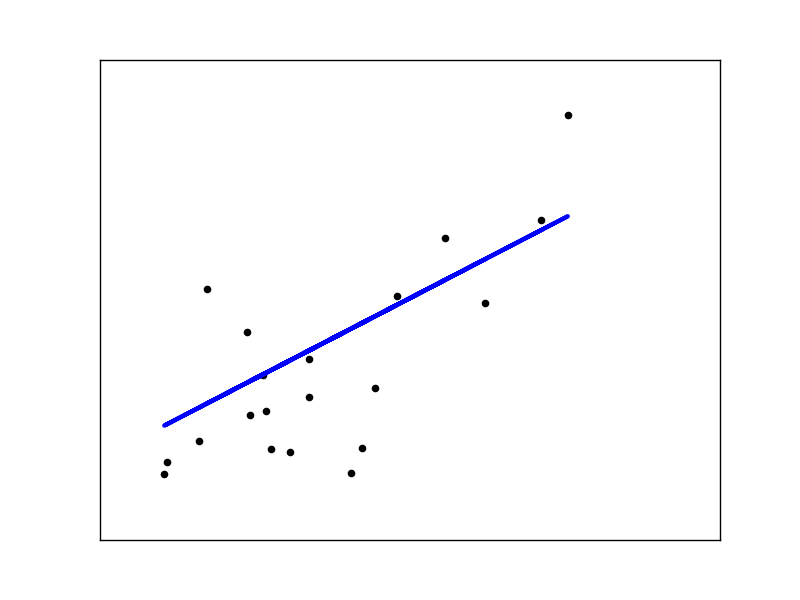
\includegraphics[height=3.5in]{figures/regression.png}
			\caption{Regresión lineal}
		\end{center}
		
		\label{regression}
	\end{figure}

	La \textbf{regresión lineal} es un modelo matemático que trata de hallar la \textbf{función lineal} que mejor se ajusta a un conjunto de puntos dispersos conocidos.
	
	Al conocer dicha función lineal, podremos \textbf{'predecir'} con un cierto grado de exactitud, lo que pasará.
	
	La línea recta que se puede ver en la gráfica \ref{regression}, muestra cómo la \textbf{regresión lineal} intenta dibujar una línea recta que minimice mejor la suma residual de cuadrados entre las respuestas observadas en el conjunto de datos, y las respuestas predichas por la aproximación lineal.
	También se calculan los coeficientes, la suma residual de cuadrados y el puntaje de varianza.
	
	\subsection{Clasificación}
	El término \textbf{clasificador} se utiliza en referencia al algoritmo utilizado para asignar un elemento entrante no etiquetado en una categoría concreta conocida. Dicho algoritmo, permite pues, ordenar o disponer por clases elementos entrantes, a partir de cierta información característica de estos.
	
	\subsection{Redes Neuronales}
	
	\begin{figure}[htb]
		
		\begin{center}
			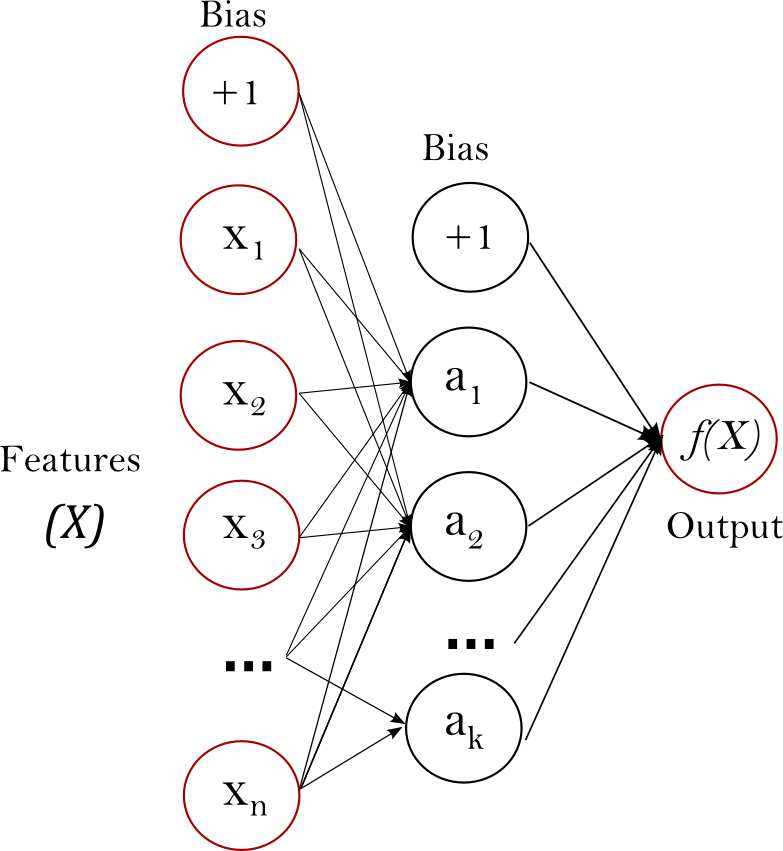
\includegraphics[height=4.5in]{figures/neuronal_network.png}
			\caption{Red neuronal}
		\end{center}
		
		\label{network}
	\end{figure}

	Las \textbf{redes neuronales} son un algoritmo de aprendizaje supervisado. Suelen consistir en varias capas ocultas donde la señal se propaga de adelante hacia atrás.
	
	A partir de X características se obtiene una función f(X).
	
\section{Protocolo del estudio}
\label{makereference3.4}

\section{Modelo escogido}
\label{makereference3.5}